\documentclass[dvips,11pt]{article}

% Any percent sign marks a comment to the end of the line

% Every latex document starts with a documentclass declaration like this
% The option dvips allows for graphics, 12pt is the font size, and article
%   is the style

\usepackage[pdftex]{graphicx}
\usepackage[utf8]{inputenc}
\usepackage{url}
\usepackage{titling}
\usepackage{lipsum}
\usepackage{geometry}


% These are additional packages for "pdflatex", graphics, and to include
% hyperlinks inside a document.

\setlength{\oddsidemargin}{0.25in}
\setlength{\textwidth}{6.5in}
\setlength{\topmargin}{0in}
\setlength{\textheight}{8.5in}

\setlength{\droptitle}{-6em}   % This is your set screw

\geometry{
	a4paper,
	total={170mm,257mm},
	left=20mm,
	top=20mm,
	right=20mm,
	bottom=20mm,
}
% These force using more of the margins that is the default style

\begin{document}

% Everything after this becomes content
% Replace the text between curly brackets with your own

\title{Cmpe 462 Project Proposal \\[2mm] Movie Recommendation\\ Using Latent Factor Models}
\author{Mustafa Onur Eken}
\date{\today}

% You can leave out "date" and it will be added automatically for today
% You can change the "\today" date to any text you like


\maketitle
\section{Introduction}

In building recommendation systems, nowadays, there are two mainstream approaches: \textit{Content-Based Filtering (CBF)} and \textit{Collaborative Filtering (CF)}. 

The key idea in the former method is that we are given some structured knowledge both about users and items themselves (Items are movies in our case) and we try to discover user, item pairs that have similar feature values.

The latter method does not require any intrinsic knowledge about users and items, but instead the only information needed is that a matrix $A$ (usually sparse), where $a_{ij} \in A$ is the rating given to item $j$ by user $i$. We can attempt to fill empty entries in the matrix by two different approaches. (1) \textit{Neighborhood models} (2) \textit{Latent factor models}.

\section{Goals \& Approach}

In this project, we have obtained a dataset (provided by \textit{MovieLens}) containing 100,000 ratings (1-5) from 943 users on 1682 movies. Our objective is to discover missing entries for each user and display recommendations accordingly. We are going to assume that there are a number (\textit{say k}) of hidden factors in which people consider when rating a movie. Then by taking actual ratings into account, we discover the association between users, factors and as well as movies, factors. We will use matrix factorization methods \cite{koren,mnih} such as \textit{alternating least squares, stochastic gradient descent, probabilistic factorization} in order to build our factor matrices and compare their performances.

\begin{figure}[!ht]
	\centering
	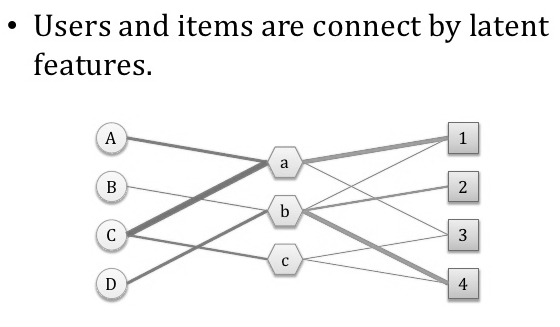
\includegraphics[width=70mm]{latent}
\end{figure}
%\section{Approach}

%The bias/variance dilemma is a problem in statistics and machine learning \cite{alpaydin}. A statistical model can not possess low bias and low variance properties (in which we ultimately desire) at the same time. It is often the case that we want our model to be detailed (large number of features) to eliminate the bias. Unfortunately, having many features in a model also brings out the problem of high variance which is undesirable if we are to make future predictions according to that model. See Figure \ref{overfitting}.

%\begin{figure}[!ht]
%	\centering
	
%	\caption{Under-fitting \& high bias (\textbf{Left}) -- Over-fitting \& high variance (\textbf{Right})}
%	\label{overfitting}
%\end{figure}
%Regularization is a method used in order to lower the variance of a detailed (over-fitting) model. There are several techniques used to achieve regularization and some of them necessitate application of a technique called Cross-validation.
%
%The fact that the dilemma mentioned above arises nearly in all machine learning applications makes regularization very important. In our presentation we will inspect and explain this topic in some depth and practically see it's effect by demonstrating an example recommending application.

\bibliography{refs}
\bibliographystyle{unsrt}



\end{document}